%%%%%%%%%%%%%%%%%%%%%%%%%%%%%%%%%%%%%%%%%%%%%%%%%%%%%%%%%%%%%%%%%%%%%%%%%%%%%%%%
%2345678901234567890123456789012345678901234567890123456789012345678901234567890
%        1         2         3         4         5         6         7         8

\documentclass[letterpaper, 10 pt, conference]{ieeeconf}  % Comment this line out if you need a4paper

%\documentclass[a4paper, 10pt, conference]{ieeeconf}      % Use this line for a4 paper

\IEEEoverridecommandlockouts                              % This command is only needed if 
                                                          % you want to use the \thanks command

\overrideIEEEmargins                                      % Needed to meet printer requirements.

% See the \addtolength command later in the file to balance the column lengths
% on the last page of the document

% The following packages can be found on http:\\www.ctan.org
%\usepackage{graphics} % for pdf, bitmapped graphics files
%\usepackage{epsfig} % for postscript graphics files
%\usepackage{mathptmx} % assumes new font selection scheme installed
%\usepackage{times} % assumes new font selection scheme installed
%\usepackage{amsmath} % assumes amsmath package installed
%\usepackage{amssymb}  % assumes amsmath package installed



\usepackage{amsmath,amssymb}

\usepackage{tikz,hyperref,graphicx,units,subfig}
\usepackage{benktools}

\usepackage{sidecap,wrapfig}
\usepackage[ruled,vlined]{algorithm2e}
\DeclareMathOperator*{\argmin}{arg\,min}
\DeclareMathOperator*{\argmax}{arg\,max}
\newcommand{\abs}[1]{\lvert#1\rvert} 
\newcommand{\norm}[1]{\lVert#1\rVert}
%\newcommand{\suchthat}{\mid}
\newcommand{\suchthat}{\ \big|\ }
\newcommand{\bd}{\mathbf{d}}
\newcommand{\bn}{\mathbf{n}}
\newcommand{\bp}{\mathbf{p}}
\newcommand{\bw}{\mathbf{w}}
\newcommand{\by}{\mathbf{y}}
\newcommand{\bx}{\mathbf{x}}
\newcommand{\bz}{\mathbf{z}}
\newcommand{\bbf}{\mathbf{f}}
\newcommand{\bzero}{\mathbf{0}}
\newcommand{\bG}{\mathbf{G}}
\newcommand{\bA}{\mathbf{A}}
\newcommand{\bW}{\mathbf{W}}
\newcommand{\bX}{\mathbf{X}}
\newcommand{\mX}{\mathcal{X}}
\newcommand{\mD}{\mathcal{D}}
\newcommand{\mN}{\mathcal{N}}
\newcommand{\mW}{\mathcal{W}}
\newcommand{\mF}{\mathcal{F}}
\newcommand{\bZ}{\mathbf{Z}}

\newcommand{\bfc}{W}
\newcommand{\Qinf}{Q_{\infty}}
\newcommand{\st}[1]{_\text{#1}}
\newcommand{\rres}{r\st{res}}
\newcommand{\pos}[1]{(#1)^+}
\newcommand{\depth}{\operatorname{depth}}
\newcommand{\dist}{\operatorname{dist}}
\newcommand{\convhull}{\operatorname{ConvexHull}}
\newcommand{\minksum}{\operatorname{MinkowskiSum}}



\title{\LARGE \bf
Efficient Sampling for Grasp Quality Evaluation on Gaussian Process Implicit Surface Representations [v-12 09-30-2014]}


\author{Michael Laskey, Zoe McCarthy, Jeff Mahler, Florian T. Pokorny, Sachin Patil,\\  Danica Kragic, Pieter Abbeel, and Ken Goldberg}% <-this % stops a space

\newtheorem{theorem}{Theorem}

\begin{document}



\maketitle
\thispagestyle{empty}
\pagestyle{empty}


%%%%%%%%%%%%%%%%%%%%%%%%%%%%%%%%%%%%%%%%%%%%%%%%%%%%%%%%%%%%%%%%%%%%%%%%%%%%%%%%


\begin{abstract}
Gaussian Process Implicit Surface (GPIS) have emerged recently as a new Bayesian shape representation.  %%PA: not sure what "Bayesian shape represenation" means -- isn't it just a distribution over shapes that it represents, which happens to allow for performing Bayesian inference?  language not very precise I guess...
Former methods for grasp evaluation with shape uncertainty require sampling from  distributions on shape. The standard approach of drawing samples from a GPIS in 2D by means of a %%PA: a -> an
 evaluation on a uniform grid has a complexity of $O(n^6)$(2D) and $O(n^9)$ in the number of grid steps $n$.%%PA: grouping of words should try to make things easier to read/follow along; does 2D only apply to the O(n^6) or to the entire sentence?  aside from sentence structuring, it's hard to understand this previous sentence, what is the n^9 about? what is a grid step?  does it mean number of discretization levels for dimension?
%%PA: also, why ".." rather than "." to end the sentence?
We propose an alternative approximation%%PA: grouping of words is off; it's not an alternative approximation, it 's an alternative to sampling from shape distributions ..
 to sampling from shape distributions and demonstrate how that reduce complexity from $O(n^6)$ in 2D and $O(n^9)$ in 3D to $O(n^3)$ for evaluation of a single grasp. 
%%PA: how about including some intuition about what the alternative is / what main idea it is leveraging?
We furthermore introduce the idea of adaptive sampling in this context by formulating it as a multi-arm bandit problem for speeding up the selection of the highest quality grasp in a set of proposed grasps.  %%PA: --> cool!!
\end{abstract}
%%%%%%%%%%%%%%%%%%%%%%%%%%%%%%%%%%%%%%%%%%%%%%%%%%%%%%%%%%%%%%%%%%%%%%%%%%%%%%%%
\section{Introduction}

\vspace{10pt}

%%PA: this citation type-setting is a bit funny to me, I am much more used to [12, 8, 10] or [12], [8], [10] rather than the current paper's typesetting as [12] [8] [10].  If you have seen it in a reputable place and it's the style you guys prefer then I am fine with it, of course
%%ZM: will fix as going through

\todo{Get High res GPIS visualizations, Incorporate next round of feedback}
Consider a robot packing boxes in a shipping warehouse environment. The robot will frequently encounter objects that it has not seen before. The robot will have to plan stable grasps without any prior information other than its sensor data. As seen in Fig. \ref{fig:noisy data}, with today's RGB and depth sensors, surface properties, such as specularity and transparency, can greatly effect the returned observations. Grasp planners based on deterministic algorithms are not designed to handle such noise and could fail. To plan grasps in a partially observed world, recent research has focused on incorporating uncertainity%%PA: --> spelling
 in the shape of the object \cite{kehoe2012estimating}, \cite{christopoulos2007handling}, \cite{zheng2005}. %%PA: why two dots? %%PA: and same paper is cited twice... %% ZM fixed

While past work has encoded uncertainty in a polygonal mesh representation \cite{kehoe2012estimating}, an alternative is to work with the signed distance fields (SDFs), a continuous valued function that is an implicit surface: zero-valued at the surface of the object, positive value outside the surface and negative valued inside the surface. This representation is growing in popularity in the robotics field for its ability to integrate range data in real time \cite{newcombe2011kinectfusion}\cite{curless1996volumetric}. To incorporate uncertainty one can use a Gaussian Process Implicit Surface (GPIS), a Gaussian process over signed distance field. Not only does GPIS present a straightforward and formal way to incorporate measurements from visual, laser and tactile sensors, they  also allow for a continuous differentiable function on shape, 
%%PA: continuous and differentiable (which I believe would be a redundant statement as differentiable implies continuous), or continuously differentiable?
which can be used for a feedback grasp controller, finding locally optimal grasps and active exploration  \cite{dragiev2011}, \cite{jeffs}, \cite{hollinger2013}. 
 
\begin{figure}[ht!]
\centering
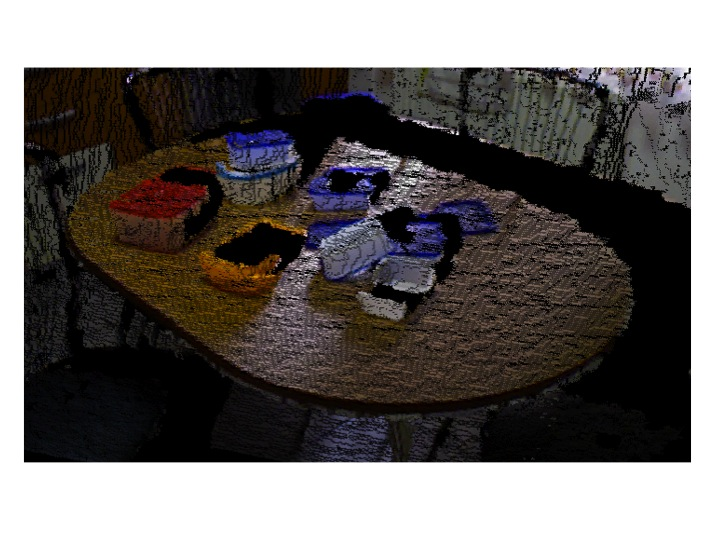
\includegraphics[width=8.5cm,height=4cm]{figures/Slide02.jpg}
\caption{Left: HD image of a common measuring cup from in a household environment. Right: Image taken from PR2's Primesense Carmine sensor, large parts of the measuring cup are not detected by the depth sensor and are not visible in the RGB image.}
\vspace*{-10pt}
\label{fig:noisy data}
\end{figure}

Given a method to represent shape uncertainty, a common technique to evaluate grasp quality is to sample from the distribution on shape and perform Monte-Carlo integration on a given grasp metric \cite{kehoe2012estimating}, \cite{kehoe2012toward}, \cite{christopoulos2007handling}. Applying this technique to GPIS requires an exhaustive sampling of the signed distance field, which scales $O(n^6)$ for a 2D $n \times n$ workspace and $O(n^9)$ for a 3D workspace.The computationally complexity of sampling is derived from the fact sampling from a Gaussian requires matrix inversion of the entire signed distance field. Our paper reduces this complexity to $O(n^3)$ by using the insight that for grasp quality evaluation one only cares about the parameters that define a grasp: contacts points, surface normals, center of mass and friction coefficient \cite{pokorny2013classical}. 
%%PA: that's neat!  let's have you include some of that in the abstract!
%%PA: also n^3 independent as to whether it's a 2-D or 3-D problem, or is n^3 specific to a particular dimensionality?
We constrain the contact points by considering the approach trajectory of a gripper.  Hence, sampling the whole signed distance field is not needed, but instead one can only work with the distributions on grasp parameters given the shape uncertainty model and gripper trajectory. In light of this our contributions are the following:
 
\begin{enumerate}
	\item Derivation of  distributions on grasp parameters given GPIS shape uncertainty model and approach trajectory of gripper.%%PA: grammar off
	\item  Demonstrating both theoretically and empirically how those distributions reduce the computational complexity of sampling.%%PA: -> computational %%ZM: fixed
	\item Applying adaptive sampling techniques to efficiently find high quality grasps in a given set of proposed grasps. 
\end{enumerate}
 
\section{Related Work}

 Past work on grasping under uncertainty has focused on state uncertainty \cite{goldberg1990bayesian}, \cite{goldberg1990stochastic}, \cite{stulp2011learning},  uncertainty in object pose \cite{christopoulos2007handling}, \cite{felip2009robust}, \cite{kim2012physically} or uncertainty in the location of contact with the object \cite{zheng2005}. Robust grasp selection for parallel jaw grippers on uncertain shapes was studied by Kehoe et al. for both zero-slip push grasps \cite{kehoe2012toward} and slip push grasps \cite{kehoe2012estimating} using Monte Carlo integration for the expected grasp quality, but this approach was limited to polygonal shapes.  Christopoulo et al. sampled spline fits for 2-dimensional planar objects to measure the quality of uncertainty, however it is has not been shown how a spline based method could incorporate non-visual sensing information for representing shape uncertainty.
 
 The choice of using Gaussian Process Implicit Surfaces to represent uncertainty, is based on the fact it provides a formal way to include various sources of noise from observations such as tactile, laser and visual. Futhermore, implicit surface representations are becoming increasingly popular in robotics due to their success in real-time surface modeling from range images \cite{curless1996volumetric}, \cite{newcombe2011kinectfusion}, \cite{hornung2013octomap}. Some exciting work done with GPIS representation are the following: Hollinger et al. used GPIS to perform active sensing on the hulls in underwater boats \cite{hollinger2013}. Dragiev et al. showed how GPIS can represent shapes for grasps and used  as a grasp controller on the continuous signed distance function \cite{dragiev2011}. Mahler et al. used GPIS representation to find locally optimal grasps by framing grasp planning as an optimization problem \cite{jeff}. %%PA: locally optimal anti-podal grasps?
 
  For grasp quality evaluation with shape uncertainty a common method involves sampling from the distribution on shape \cite{kehoe2012estimating}, \cite{kehoe2012toward}, \cite{christopoulos2007handling}. With GPIS this requires computationally intensive sampling from a signed distance field that is the dimension of the workspace. We propose an alternative distribution to sample from, based on the idea that we only need to consider the approach trajectory of the gripper. 

Monte-Carlo integration involves drawing random samples from a distribution to approximate an integral \cite{caflisch1998monte}. While previous work has looked at quality evaluation of a single grasp with uncertainty \cite{christopoulos2007handling}, \cite{zheng2005}, few have compared many different grasps with uncertainty and efficiently chosen the best one.  Adaptive Sampling is the idea of allocating samples based on previous observations or rewards, which can be described as a multi-arm bandit problem \cite{barto1998reinforcement}. Prior work by Kehoe et al. \cite{kehoe2012toward} used an adaptive sampling approach that removed low quality grasps based on values received, but this method had no statistical guarantees and could lead to high quality grasps being removed. To achieve guarantees, we frame the problem as a "budgeted multi-arm bandit" problem, where exploration and exploitation are decoupled and the agent has to allocate resources to explore for a finite time then decide which arm to exploit  \cite{madani2004budgeted}. Drawing from the literature on Monte-Carlo sampling we estimate the confidence bounds of grasps and prune only those that are statistically distinguishable \cite{caflisch1998monte}.  



\section{Preliminaries and Problem Statement}

In this section we describe the mathematical derivation of Gaussian Process Implicit Surface representations.

\subsection{Gaussian Process (GP) Background}
GPs provide an infinite dimensional analogue of Multivariate
Gaussian Distributions which allow us to model distributions over
functions. Gaussian processes (GPs) are widely used in machine learning as a nonparametric regression method for estimating continuous functions from sparse and noisy data \cite{rasmussen2010gaussian}.
In a GP, a training set consists of input vectors $\mX = \{\bx_1, \ldots, \bx_n\}$, $\bx_i \in \mathbb{R}^d$, and corresponding observations $\by = \{y_1, \ldots, y_n\}$. The observations are assumed to be noisy measurements from the unknown target function $f$:
\begin{equation}
y_i = f(\bx_i) + \epsilon,
\end{equation}
where $\epsilon \sim \mN(0,\sigma^2)$ is Gaussian noise in the observations.
A zero-mean Gaussian process is completely specified by a covariance function $k(\cdot,\cdot)$, also referred to as a kernel.
Given the training data $\mD = \{\mX, \by\}$ and covariance function $k(\cdot,\cdot)$, the posterior density $p(f_*|\bx_*,\mD)$ at a test point $\bx_{*}$ is shown to be \cite{rasmussen2010gaussian}:
\begin{align*}
	p(f_*|\bx_*,\mD) &\sim \mN\big(\mu(\bx_*), \Sigma(\bx_*)\big) \\
	\mu(\bx_*) &= k(\mX,\bx_*)^{\intercal}(K + \sigma^2I)^{-1}\by \\
	\Sigma(\bx_*) &= k(\bx_*,\bx_*)-k(\mX,\bx_*)^{\intercal}(K+\sigma^2I)^{-1}k(\mX,\bx_*)\big) 
\end{align*}
where $K \in \mathbb{R}^{n \times n}$ is a matrix with entries $K_{ij} = k(\bx_i,\bx_j)$ and $k(\mX,\bx_*) = [k(\bx_1,\bx_*),\ldots,k(\bx_n,\bx_*)]^{\intercal}$. 
This derivation can also be used to predict the mean and variance of the function gradient by extending the kernel matrices using the identities \cite{solak2003derivative}:

\vspace{-2ex}
\begin{align}
	\text{cov}\left(f(\bx_i), f(\bx_j) \right) &=  k(\bx_i, \bx_j) \\
	\text{cov}\left(\frac{\partial f (\bx_i)}{\partial x_k}, f(\bx_j) \right) &= \frac{\partial}{\partial x_k} k(\bx_i, \bx_j) \label{eq:mean_gradient}\\
	\text{cov}\left(\frac{\partial f (\bx_i)}{\partial x_k}, \frac{\partial f (\bx_j)}{\partial x_l} \right) &= \frac{\partial^2}{\partial x_k \partial x_l} k(\bx_i, \bx_j)\label{eq:cov_gradient}
\end{align}

\begin{figure}[ht!]
\centering
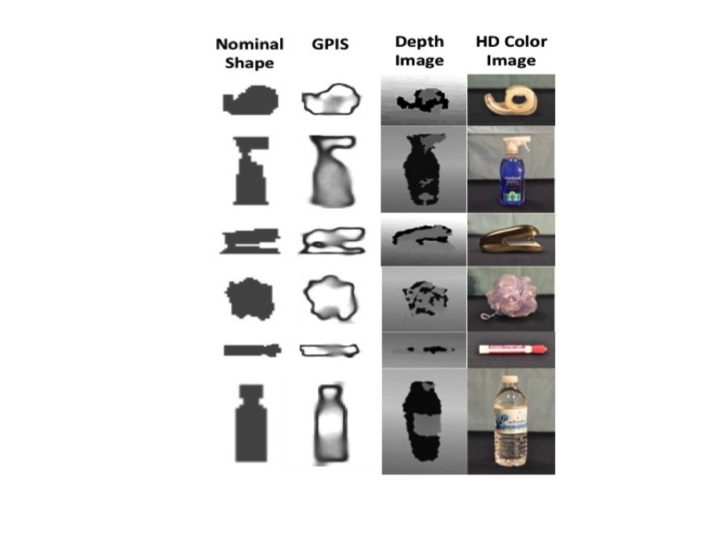
\includegraphics[width = 8.5cm, height = 14cm ]{figures/Slide03.jpg}
\caption{Six example objects illustrating transparency, specularity, sensor noise that illustrate the need for shape uncertainty: (from top to bottom) tape, squirt bottle, stapler, loofa, marker, water bottle. Displayed from right to left are the HD color image, a point cloud observation from a Primesense Carmine, GPIS visualization technique from \cite{jeffs}, the nominal shape on a $25 \times 25$ grid.  }
\vspace*{-10pt}
\label{fig:GPIS_TSDF}
\end{figure}
%\section{Related Work}

For our kernel choice we decided to use the square exponential kernel, a major reason for this was its differentiability. Other kernels relevant to GPIS are the thin-plate splines kernel and the Matern kernel \cite{williams2007}. %%PA: motivation seems a little weak; did you compare performance with other kernels? (must be other differentiable ones?) could something be added about why differentiability is important to our approach?

We construct a GPIS by learning a Gaussian Process to fit measurements of a signed distance field of an unknown object.  Precisely, $x_i \in \mathbb{R}^2$ in 2D and $x_i \in \mathbb{R}^3$ in 3D, and $y_i \in \mathbb{R}$ is a noisy signed distance measurement to the unknown object at $x_i$.



\subsection{Line of Action}
Similar to the work of \cite{christopoulos2007handling}, we assume that each gripper finger approaches along a \textit{line of action}, a 1D curve $\gamma(t)$ with endpoints $a$ and $b$ as seen in Fig. \ref{fig:line_of_action}. A gripper finger starts at point $a$ and moves towards $b$, we assume $a$ is far enough away to be collision free of the object.  Each gripper contact is defined by a line of action, so we assume the following tuple is provided $\Gamma = ( \gamma_1(\cdot),...,\gamma_m(\cdot) )$, which designates a proposed \textit{grasp plan}. 

\begin{figure}[ht!]
\centering
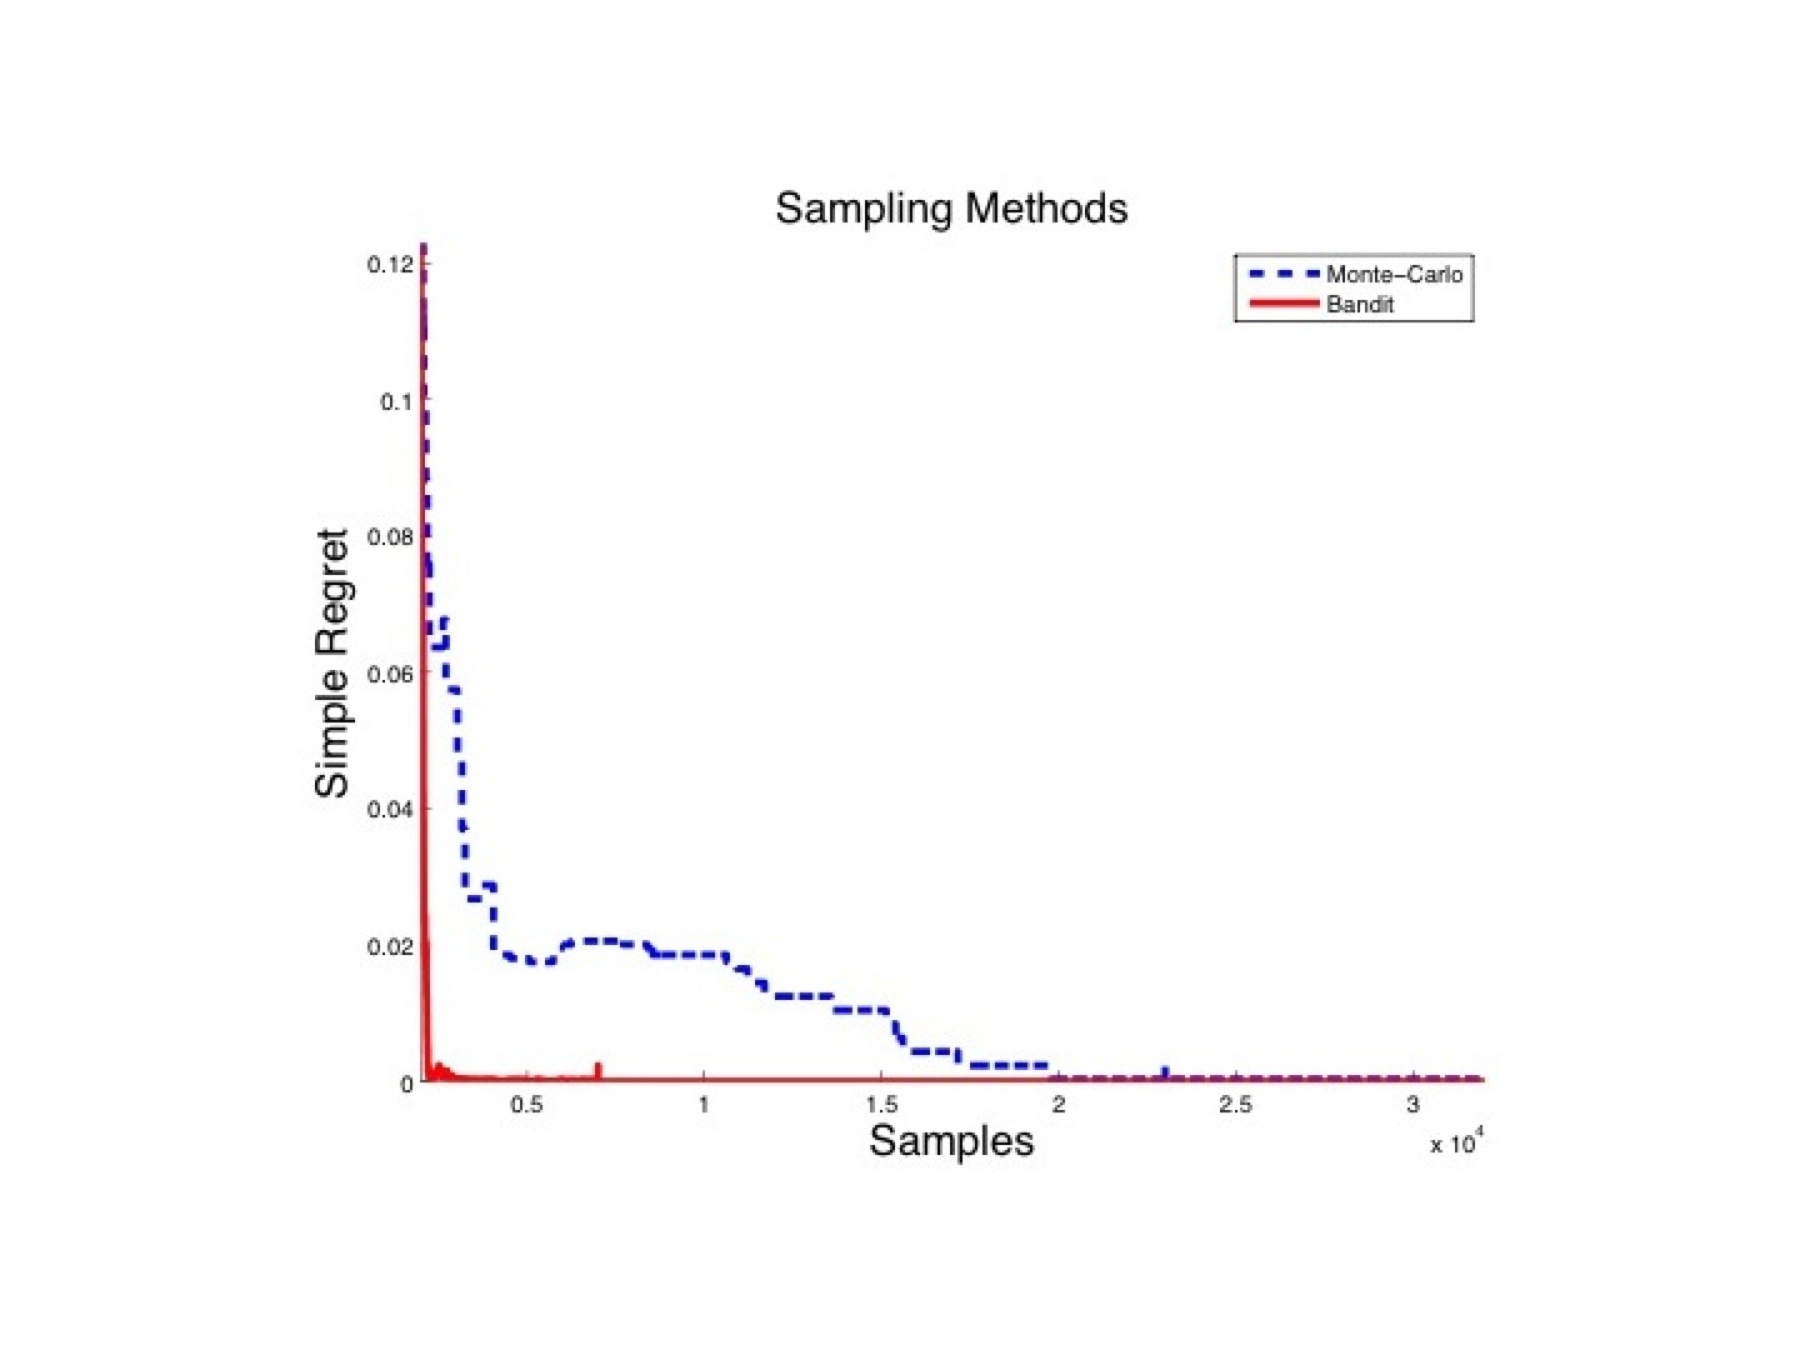
\includegraphics[scale = 0.3]{figures/Slide01.jpg}
\caption{Illustration of a grasp plan $\Gamma$ composed of two lines of action, $\gamma_1(t)$ and $\gamma_2(t)$}
\vspace*{-10pt}
\label{fig:line_of_action}
\end{figure}

\subsection{Problem Definition}

Given a 2-D workspace $\mathcal{W}$, with an unknown object represented as a trained GPIS model and set of possible grasp plans $G$. We are interested in determining 

\begin{align}\label{eq:problem_def}
\Gamma^* \in \mbox{argmax}_{\Gamma \in G} E(Q(\Gamma))
\end{align}

with respect to a chosen grasp metric Q. 

\section{Evaluating a Grasp}
In order to solve our problem definition, we must evaluate $E(Q(\Gamma))$ for a given grasp plan $\Gamma$. We will first discuss which grasp metric $Q$ we chose and then proceed into evaluating the expectation $E$ efficiently. 

\subsection{Grasp Metric}
In their pioneering work over two decades ago Ferrari and Canny \cite{ferrari1992}, demonstrated a method to rank grasps by considering their contact points and surface normals. Importantly the magnitude of Q yields a measurement that allows one to rank grasps by their physical stability and evaluate the property of force-closure. Furthermore, it has wide spread use in grasp packages like GraspIT\cite{miller2004graspit}, OpenGrasp\cite{73} and Simox \cite{vahrenkamp2010simo}, which motivates studying its effect with uncertainties. 

The $L^1$ version of the metric works by taking as input the contact points $\textbf{c}_1,...,\textbf{c}_m$, surface normals $\textbf{n}_1,...,\textbf{n}_m$, center of mass $z$ and friction coefficient $\mu$. Then constructing a convex hull around the wrenches made up of those parameters and finding the radius of the largest unit ball centered at the origin in wrench space. A wrench is defined as concatenation of a force and torque vector.  If the convex hull doesn't enclose the origin, the grasp is not in force-closure. Thus a grasp can be parameterized by the following tuple $g = \lbrace \textbf{c}_1,...,\textbf{c}_m,\textbf{n}_1,...,\textbf{n}_m,\mu, \textbf{z} \rbrace$, our method is applicable to all grasp metrics that represent a grasp as the tuple $g$, such as \cite{christopoulos2007handling}, \cite{li1988task}. 

\subsection{Calculating the Expected Grasp Quality}
Given a proposed grasp plan $\Gamma$, the expected grasp quality can be evaluated as follows:

\vspace{-2ex}
\begin{align}\label{eq:shape_sampling}
E(Q(\Gamma)) = \int Q(g|S,\Gamma) p(S) dS
\end{align}



Where $Q(g|S,\Gamma)$ is the grasp quality that is computed on a shape sample drawn from $p(S)$. To compute this we intersect the zero crossing of the level set with the propose grasp plan $\Gamma$ and determine the parameters $g$, this has been the approach taken in previous work  \cite{kehoe2012estimating} \cite{kehoe2012toward} \cite{christopoulos2007handling}. See Fig. \ref{fig:shape_samples} for an example of what samples drawn from $p(S)$ induced by GPIS look like. For computational reasons we approximate the integral via Monte-Carlo Integration. We use importance sampling to draw from the distribution induced by GPIS and calculate the following

\begin{figure}[ht!]
\centering
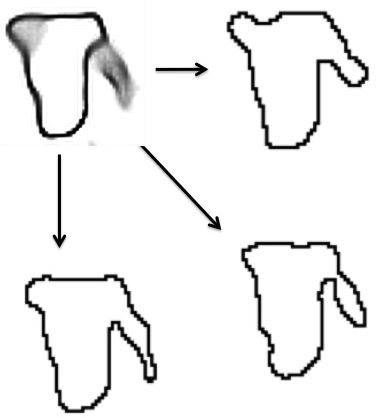
\includegraphics[width = 8.5cm, height= 5cm ]{figures/Slide13.jpg}
\caption{Shape samples drawn from Eq. \ref{eq:joint_shape} on the object in the upper left corner. Given a shape sample we highlight the zero-crossing of the level set in black}
\vspace*{-10pt}
\label{fig:shape_samples}
\end{figure}

\begin{align*}
E(Q(\Gamma)) \approx \sum_{i=1}^N Q(g|S_i,\Gamma) , S_i \in p(S) %%PA: 1/N missing?
\end{align*}

To compute the above distribution we must draw samples from $p(S)$. In order to draw shape samples from a GPIS, one needs to sample from signed distance function, $sd$, over the joint on all points in the workspace $\mathcal{W}$ or $p(sd(\mathcal{W}))$. Since this is a GPIS, we know the following 

\begin{align}\label{eq:joint_shape}
p(S) = p(sd(\mathcal{W})) \sim N(\mu(\mathcal{W}),\Sigma(\mathcal{W}))
\end{align}

Thus if the workspace is an $n \times n$ grid, the joint distribution is an  $n^2$ multi-variate Gaussian, due to $sd:\mathbb{R}^2 \rightarrow \mathbb{R}$.  Sampling from a Gaussian involves inverting the covariance matrix and inversion is in the naive way $O(n^3)$ \cite{petersen2008matrix}. %%PA: that last use of $n$ has a different meaning, that's confusing, use a different symbol than n, or just say in words it's cubic in the number of grid points
Thus the complexity of this operation is $O(n^6)$ in 2D and $O(n^9)$ in 3D. 

To reduce complexity we propose sampling not from the shape distributions, but instead from the distributions on the grasps parameters themselves. We recall that a grasp according to our metric is defined as the tuple $g = \lbrace \textbf{c}_1,...,\textbf{c}_m,\textbf{n}_1,...,\textbf{n}_m,\mu, z \rbrace$. We are thus interested in calculating $p(g|\Gamma,\mu(x),\Sigma(x))$. The distribution on a grasp is defined then as: 

\begin{align}\label{eq:joint_on_shape}
p(g) = p\big(\textbf{c}_1,...,\textbf{c}_m,\textbf{n}_1,...,\textbf{n}_m|\Gamma,\mu(x),\Sigma(x)\big)
\end{align}

We note here that we currently use the friction coefficient $\mu$ and the expected center of mass $\bar{z}$ as deterministic values. For grippers that do not approach along the same line of action (i.e. non-parallel jaw grippers) we make the assumption that each contact and normal pair is independent, or 

\vspace{-2ex}
\begin{align}\label{eq:independence}
p(g) = &\prod_{i=1}^mp\big(\textbf{c}_i,\textbf{n}_i|\gamma_i(t),\mu(x),\Sigma(x)\big)
\end{align}



We compute the expected grasp quality now as follows: 

\vspace{-2ex}
\begin{align}\label{eq:grasp_sampling}
E(Q(\Gamma)) = \sum_{i=1}^N Q(g_i) , g_i \in p(g)
\end{align}


We will now show how these distributions can be computed and how the complexity for evaluating a grasp is reduced from $O(n^6)$ to $O(n^3)$. 


\section{Distribution of Grasp Parameters}
\label{sec:distgrasp}
 
 To sample from $p(g)$, we need to compute the distributions associated with a line of action $p(n_i|c_i)p(c_i|\gamma_i(t),\mu(x),\Sigma(x))$ on each of the parameters: contact points $c_i$, surface normals $n_i$  and expected center of mass $\bar{z}$. 
 .
\subsection{Distribution on Contact Points} 
The probability distribution along the line $\gamma(t)$ is given by:

\vspace{-2ex}
\begin{equation} \label{eq:line_of_act_dist}
p\big(sd(\gamma(t)) ; \mu(t),\Sigma(t)\big) \ \forall t \in [a,b] 
\end{equation}

This gives the signed distance function distributions along the entire line of action in the workspace as a multivariate Gaussian. One could think of this as a marginalization of all other points in signed distance field except the line of action. We would like to find the distribution on the first contact point, which we can define as when the signed distance function $sd(\gamma(t))$ is $0$ and all previous times $\tau$ we have $sd(\gamma(\tau)) > 0$ for all $\tau$ such that $0 \leq \tau < t$.We thus compute this as the joint distribution $p\big( \textbf{c}_i= \gamma(t)\big) = p\big(sd(\gamma(t))=0, sd(\gamma(\tau))> 0 \big)$ $  \forall \tau \in [0,t)$.

We now derive this distribution: 

\vspace{-2ex}
\begin{align}
 & p\big(\textbf{c}_i = \gamma(t)\big) = \label{eq:contact_theory} \\
  & \frac{1}{\eta} p\big(sd(\gamma(t)) = 0\big)P\big(sd(\gamma(\tau)) > 0 | sd(\gamma(t)) = 0\big) \\
  & \forall \tau \in [0,t)
\end{align}


Where $\eta$ is a proportionality constant. The first product in the equation can be computed easily using the marginalization of a multivariate Gaussian distribution and the second term can be solved by first conditioning on the joint $p(sd(\gamma(t))|sd(\gamma(t)) = 0)$ and then computing the cumulative distribution function  \cite{petersen2008matrix}.  We show the theoretical distribution on $\textbf{c}_i$ calculated for a given GPIS and line of action in Fig.
\ref{fig:GraspDist}.

\begin{figure*}[ht!]
\centering
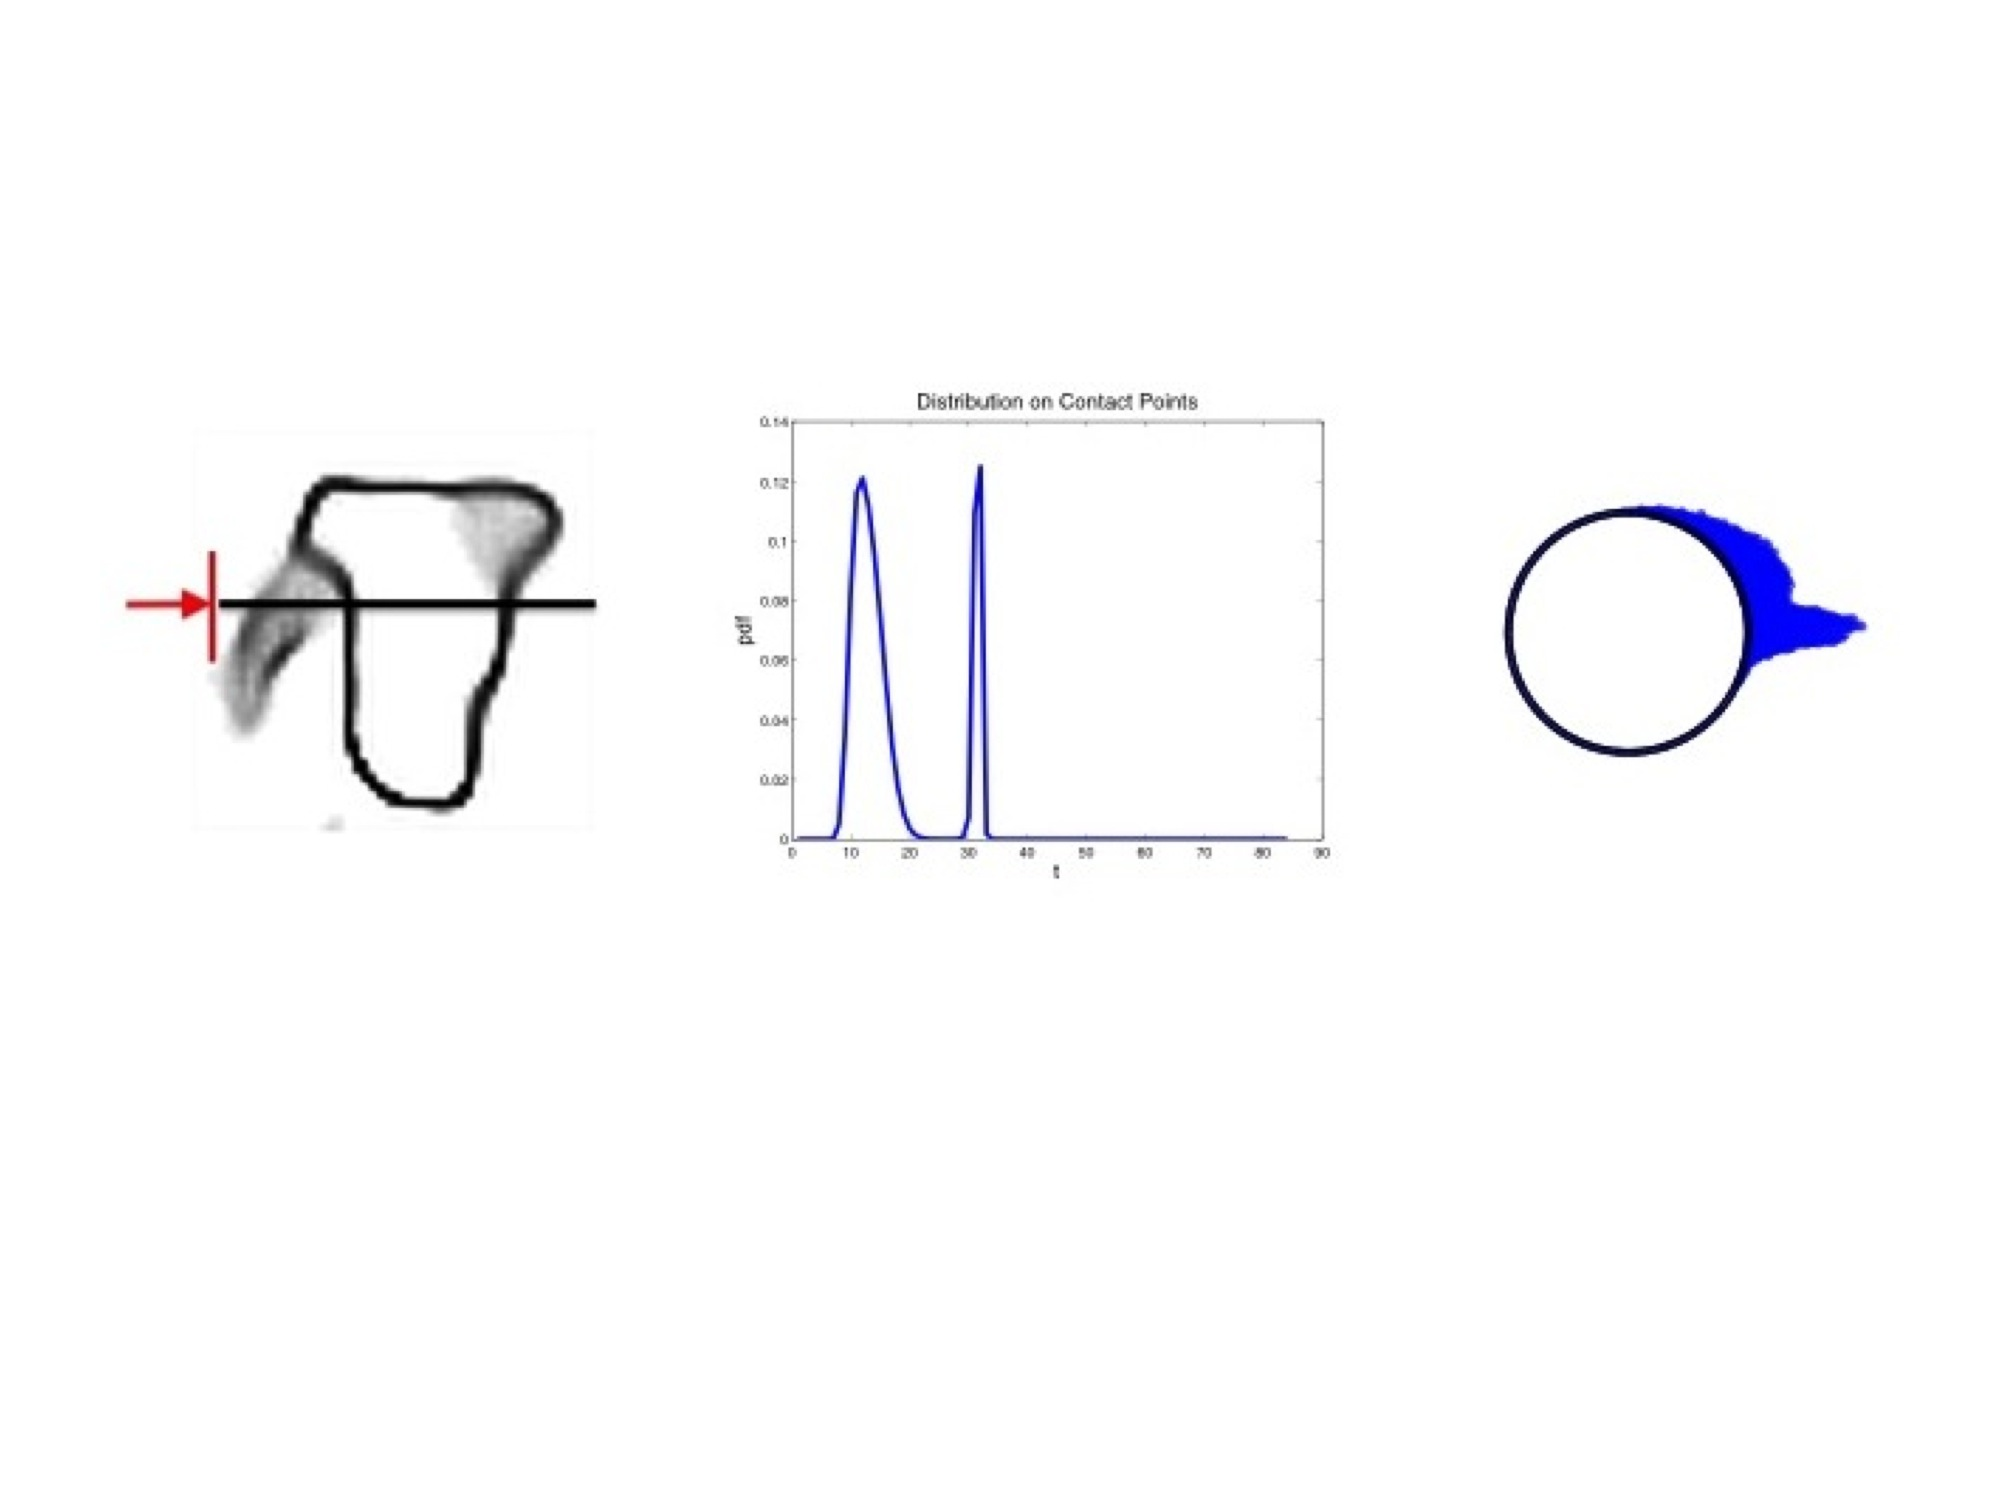
\includegraphics[width = 17cm, height = 4.5cm]{figures/Slide04.jpg}
\caption{(Left to Right): Line of action for a given gripper on an uncertain surface representing a measuring cup. Distribution $p(c)$ as a function of $t$, the position along the line of action $\gamma(t)$. The two modes correspond to the different potential contact points, either the handle or the base of the cup. Lastly, the distribution on the surface normals (inward pointing) along $\gamma(t)$ described by equation \ref{eq:normal_dist}. }
\vspace*{-10pt}
\label{fig:GraspDist}
\end{figure*}

In practice Eq. \ref{eq:contact_theory} is not efficient to compute because it requires computation of the cumulative distribution function of a large multivariate Gaussian, so instead we sample from Eq. \ref{eq:line_of_act_dist} and find the first positive to negative zero-crossing of the sample along the line. 


%%PA: it's not clear to me where the savings are coming from; the goal was to avoid sampling from the GPIS; but now it seems the algorithm needs to sample from the GPIS after all to obtain the grasp parameters?  What am I missing here?  Please address not just in the paper, but also via email

%%PA: if you are indeed avoiding sampling from th GPIS now, then it'd be good to highlight that, and explain exactly how that was enabled...

%%PA: the entire Section V. is a bit confusing; reads very procedural, but not a very clean straightforwardly explained procedure, and the rationale / context / big idea is not explained...


\subsection{Distribution on Surface Normals} 
Using Eq. \ref{eq:mean_gradient} and Eq. \ref{eq:cov_gradient}, we can compute the mean of the gradient $ \mu_{\nabla}(x)$ and the covariance of the gradient $\Sigma_{\nabla}(x)$ respectively. Thus we can compute the distribution around the surface normal for a given point in $\mathcal{W}$. We can now write 

\vspace{-2ex}
\begin{align*}
p\big(\textbf{n}_i|\textbf{c}_i = \gamma(t)\big) = p\big(\textbf{n}_i |\mu(\gamma(t)), \Sigma(\gamma(t)) \big)
\end{align*}

One interesting effect of this technique is that we can now marginalize out the line of action model and visual what the surface normal distribution is along a given line of action. To our knowledge this is the first attempt to visual surface normals along a grasp plan. Marginalization can be performed as follows:

\vspace{-2ex}
\begin{equation}
p(\textbf{n}_i ) = \int_a^b   p\big(\textbf{n}_i = \textbf{v} | \textbf{c}_i = \gamma(t) \big)p\big(\textbf{c}_i = \gamma(t)\big) dt
\end{equation}

Grasp metrics such as  Ferrari-Canny require $\textbf{n}_i$ be normalized, or, equivalently, a member of the sphere $\mathcal{S}^{d-1}$ \cite{ferrari1992}. To account for this we densely sample from the  distribution $p \big(\textbf{n}_i ) \big)$  and project onto $\mathcal{S}^{d-1}$.  In Fig.\ref{fig:GraspDIst}, we visualize the theoretical distribution on $\textbf{n}_i$ calculated for a given GPIS and approach line of action.


\subsection{Expected Center of Mass} 

We recall the quantity $P(sd(x) < 0) = \int_{-\infty}^{0} p(sd(x) =  s \ | \ \mu(x),\Sigma(x)) ds$ is equal to the probability that $x$ is interior to the surface under the current observations.
We assume that the object has uniform mass density and then $P(sd(x) < 0)$ is the expected mass density at $x$.
Then we can find the expected center of mass as:

\begin{equation}
  \bar{z} 
  =
  \frac
    {\int_{\mathcal{W}}x P(sd(x)<0) dx}
    {\int_{\mathcal{W}}  P(sd(x)<0) dx}
\end{equation}

which can be approximated by sampling $\mathcal{W}$ in a grid and approximating the spatial integral by a sum. Since this operation involves the entire SDF, one would want to use a low resolution grid for computational efficiency. We show the computed density and calculated expected center of mass for a marker in Fig. \ref{fig:GPIS_MASS}.


\begin{figure}[ht!]
\centering
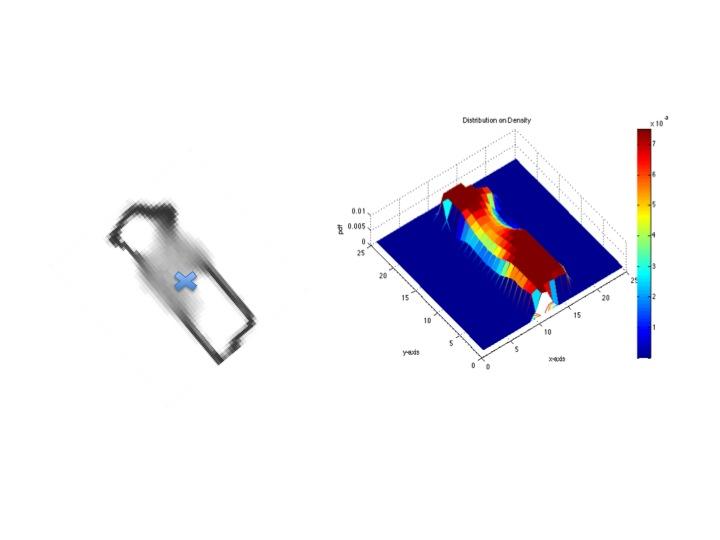
\includegraphics[scale = 0.3]{figures/Slide06.jpg}
\caption{Left: A surface with GPIS construction and expected center of mass (black X)
Right: The distribution on the density of each point assuming uniform density}
\vspace*{-10pt}
\label{fig:GPIS_MASS}
\end{figure}

\subsection{Complexity Analysis on Sampling From Grasps Distributions}

After formally deriving each distribution,  we can now sample along each line of action $\gamma_i(t)$ from the joint distribution $p(\textbf{c}_i,\textbf{n}_i | \gamma_i(t))$, due to our independence assumption Eq. \ref{eq:independence}. This can be done by drawing samples from Eq. \ref{eq:joint_contact_normal}. and using our projection technique for the normal distribution. 

Having a distribution along a line of action model allows us to sample from those instead of the joint distribution $p(sd(\mathcal{W}))$. Assuming the line of action is on the order of $n$, sampling from this distribution for a single grasp is $O(n^3)$. However, each proposed grasp plan $\Gamma$ requires the distribution to be computed, so if we have $T=|G|$ then the complexity is $O(Tn^3)$. In practice, this should be much smaller than $O(n^6)$. 

\section{Adaptive Sampling for Grasp Selection}
After determining how to efficiently compute the $E(Q(\Gamma))$, we need to now compute the full problem of Eq. \ref{eq:problem_def}, hence the selecting the best grasp plan $\Gamma^*$. While a standard approach to solving this problem would be to simply perform Monte-Carlo integration on each $\Gamma_i$ and compute the expected grasp quality, we propose treating the problem as a multi-arm bandit problem and forming a policy for selecting which grasp to sample. The motivation behind this is due to the expensive evaluation that our grasp metric Q can take \cite{ferrari1992} and the fact that the convergence of the expected quality of a typical grasp can take hundreds of evaluations as shown in Fig. \ref{fig:sampling_convergence}.  %%PA:-> grammar?

\begin{figure}[ht!]
\centering
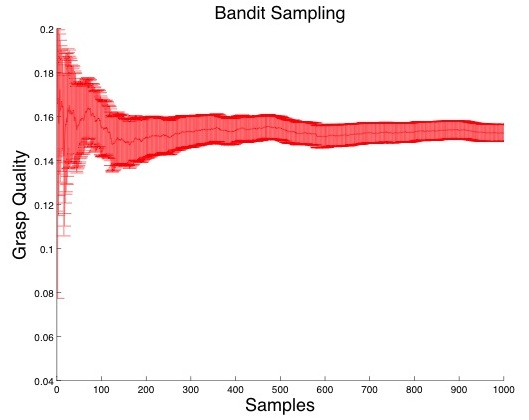
\includegraphics[width=8.5cm,height=9cm]{figures/Slide11.jpg}
\caption{Convergence of expected grasp quality, $E(Q(g))$,  for a typical grasp. You can see it can take hundreds of evaluations to correctly estimate the expected grasp quality, thus it is important to  intelligently allocate sampling resources}
\vspace*{-10pt}
\label{fig:sampling_convergence}
\end{figure}


\subsection{Preliminaries}
Compared to classical multi-arm bandit problems where the agent is evaluated on cumulative reward at each time-step, we are interested in a decoupling of the exploration and exploitation stage. The decoupling is because the agent only needs to select one grasp plan $\Gamma*$ to execute after it has sufficiently explored the other grasp plans. The agent is expected to explore the states and then at a given time, stop and choose the best grasp plan. This type of pure exploration problem with a limited amount of resources (i.e. computation time) is defined as a "budgeted multi-arm bandit problem" \cite{madani2004budgeted}. 

More formally an agent is given a set prior distributions $\mathcal{P}(1,...,K)$ for the K arms based on the awards seen.%%PA: -> rewards?  
 At each interval an arm $I_t$ is pulled based on some allocation strategy $\psi_t \in \lbrace 1,...,K \rbrace$. This happens until a stopping signal is given at which point an arm (or grasp plan) is chosen based on a recommendation strategy $\zeta_t \in \lbrace 1,...,K \rbrace$. 

Performance of our polices $\psi_t$ and $\zeta_t$ are measured according to simple regret $r_t$ \cite{bubeck2009pure}. 

\vspace{-2ex}
\begin{align}\label{eq:simple_regret}
&r_t = r(\zeta_t) = \mu^* - \mu_{\zeta_t} \\
&\mu^* = \mu_j* = \max_{j=1,..,K} \mu_j
\end{align}

%%PA: hard to follow along, lots of notation, is it really necessary to introduce that many new symbols to get the point across?


As shown in Eq. \ref{eq:simple_regret}, simple regret is defined as the difference between the true expected value of the grasp plan your recommendation, $\mu_{\zeta_t}$ and the true expected value of the best grasp plan $\mu^*$ in the set $G$. 

\subsection{Our Implementation}
In solving Eq. \ref{eq:problem_def}, we want to pick the grasp plan with the highest $E(Q(\Gamma))$ determined via Monte-Carlo Integration. Due to the non-linear nature of our grasp metric, we currently do not have a way to represent the distribution on grasp quality of $p(Q(\Gamma))$. Thus, we are restricted to the type of bandit policies available to us.

In light of this we implement our allocation policy $\psi_t$ as simple uniform allocation. This has been shown to have good performance when the number of evaluations is large \cite{bubeck2009pure}. We adapt pure uniform allocation by measuring the $95\%$ confidence interval of each arm based on previous observations.If a given arm $i$ is pulled $n_i$ times, the confidence interval $C_{n, i}$ is defined as \cite{caflisch1998monte}.

\vspace{-2ex}
\begin{align}
C_{ i} = \frac{1.96 \sigma_i}{\sqrt{n_i}}
\end{align}

%%PA: how does a single number define an interval?

%%PA: again lots of notation and symbols, how about explaining it primarily in plain words, would anything be lost? if so, introduce symbols / equations for what you lose as necessary...

%%PA: to me this doesn't sound like uniform allocation; while I can't actually follow along, my hunch is that you have confidence intervals, and at each step you consider which grasps are still in contention for being a winner based on their confidence intervals, and then sample a shape (is is a shape? is it something else that you sample?) once for each grasp

An arm $i$ is then removed from the possible options if 

\vspace{-2ex}
\begin{align*}
\mu_{\zeta_t} - C_{\zeta_t} >   \mu_{i}+C_{i}
\end{align*}

Our recommendation strategy $\zeta_t$ is to take the highest expected grasp quality at time $t$. In future work, we will look at using other allocation and recommendation strategies. 

\section{Experiments}
For the experiments below we used common household objects shown in Fig. \ref{fig:GPIS_TSDF}. We manually created a 25 x 25 grid, by tracing a pointcloud of the object on a table taken with a Primesense Carmine depth sensor. To accompany the SDF, we created an occupancy map, which holds 1 if the point cloud was observed and 0 if it was not observed, and a measurement noise map, which holds the variance 0-mean noise added to the SDF values. The parameters of the GPIS were selected using maximum likelihood on a held-out set of validation shapes. Our visualization technique follows the approach of \cite{jeffs} and consisted of drawing many shape samples from the distribution and blurring accordingly to a histogram equalization scheme. 

We did experiments for the case of two hard contacts in 2-D, however our methods are not limited to this implementation. We drew random lines of actions $\gamma_1(t)$ and $\gamma_2(t)$ by sampling around a circle with radius $\sqrt{2}n$ and sampling the circles origin, then projecting onto the largest inscribing circle in the workspace. 


\subsection{Sampling from Grasps Vs. Shape}
We first tested 1000 grasp plans and sampled each one 5000 times  and measured the RMS error between converged expected grasp plan qualities for sampling shape Eq. \ref{eq:shape_sampling} vs. grasps  Eq. \ref{eq:grasp_sampling} was 0.004. After confirming the distributions converged close to the same value, we show the computational complexity in Fig. \ref{fig:speed_dif} of the two methods for evaluating 100 grasps on an $n \times n$ grid. 

%%PA: it'd be nice to have the text be such that you can read it, and from that understand what the conclusions are from the experimentation...

\begin{figure}[ht!]
\centering
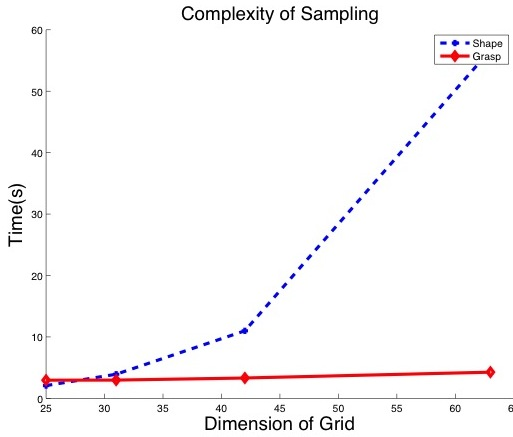
\includegraphics[width=8.5cm,height=9cm]{figures/Slide12.jpg}
\caption{Time it took to sample from 100 grasp distributions for a given resulution of the workspace. Blue line is sampling from $p(sd(\mathcal{R}))$ or shapes and Green is sampling from $p(g)$ or the calculated distribution on grasps. As you can see sampling from the calculated distributions scales much better. }
\vspace*{-10pt}
\label{fig:speed_dif}
\end{figure}





\subsection{Adaptive Sampling Technique}

We consider the problem of selecting the best grasp out of a set $G$ given a fix number of iterations $I$. For our experiments we look at selecting the best grasp out of a size of $|G| = 1000$ and $I= 7000$ or when the set of grasps is a single grasp. In Fig. \ref{fig:simple_regret}, we plotted the simple regret, Eq. \ref{eq:simple_regret}, averaged over 20 runs and compare it to the naive Monte-Carlo method that randomly chooses a grasp plan to draw a sample from . The most interesting thing is that the regret is minimized an order of magnitude faster than the naive approach, thus motivating the use of including observations as you select samples. 


\begin{figure}[ht!]
\centering
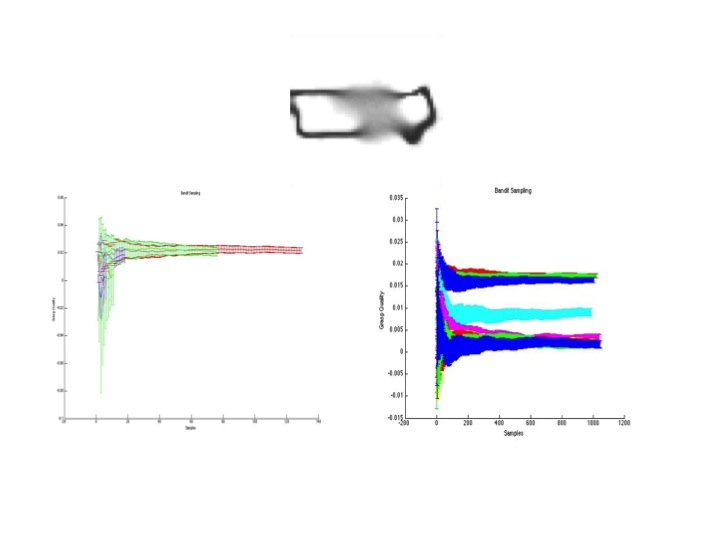
\includegraphics[width=8.5cm,height=9cm]{figures/Slide09.jpg}
\caption{Comparison of two sampling methods. Green is the adaptive bandit method that actively chooses which one to sample and Blue is the naive Monte-Carlo method. We measure their ability to converge in terms of simple regret Eq. \ref{eq:simple_regret} averaged over 100 runs. We had them determine the best grasp when $|G|=1000$. As you can see our method converges much faster with an average of evaluation of 4 samples per grasp. We start the process though by deterministically evaluating every grasp 2 times to achieve a baseline, which explains the first part of the graph.}
\vspace*{-10pt}
\label{fig:simple_regret}
\end{figure}

%%PA: was this an experiment on one shape distribution? that'd be rather anecdotal then... Did you run more extensive experiments?





\section{Limitations and Future Work}
Sampling from our distribution $p(g)$ over $p(S)$ yields a reduction in computationally complexity, but only if the number of grasps one wants to evaluate remains small relative to $n^3$, techniques to ensure this could be to find locally optimal potential grasps using optimization approaches \cite{jeffs}. 

An additional problem is that we only have an expected center of mass and not a distribution on the center of mass. This might prove to be to expensive to compute, however recent work by Panahi et al. showed a way to bound the center of mass for convex parts. Extension of his work to implicit surfaces could be of possible interest \cite{panahi2014bounding}.  

Our budgeted multi-arm bandit approach appears promising, but we still do not know how well it will perform on 3D shapes and large scale grids. Future work will be building an efficient construction of GPIS to scale to 3D. Lastly, we are interested in investigating how well our algorithm works in parallel computing to be used in the cloud computing context. Furthermore, their is a large literature on formulating bandit policies and experimenting with them all will need to be done to see which one works best. 

\bibliographystyle{ieeetr}
\bibliography{references}

\end{document}
